\documentclass[12pt]{article}

\usepackage[top=5em, bottom=5em, left=5em, right=5em]{geometry}
\usepackage{listings}
\usepackage{tikz}
\usetikzlibrary{positioning}

\setlength\parindent{0em}
\setlength\parskip{1em}

\title {Assignment 3}

\author {Hendrik Werner s4549775}

\begin{document}
\maketitle

This was done in collaboration with Constantin Blach (s4329872).

\section{} %1
Initial state:

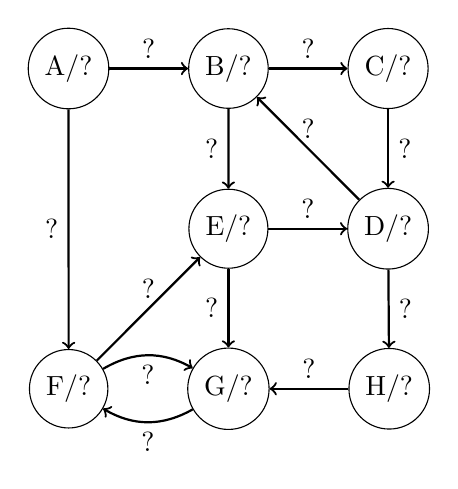
\begin{tikzpicture}[c/.style={circle, draw}]
	\node [c] (A) {A/?};
	\node [c, right=of A] (B) {B/?};
	\node [c, right=of B] (C) {C/?};
	\node [c, below=of C] (D) {D/?};
	\node [c, left =of D] (E) {E/?};
	\node [c, below=of E] (G) {G/?};
	\node [c, left =of G] (F) {F/?};
	\node [c, right=of G] (H) {H/?};

	\path[->, thick] (A) edge node [above] {?} (B);
	\path[->, thick] (A) edge node [left ] {?} (F);
	\path[->, thick] (B) edge node [above] {?} (C);
	\path[->, thick] (B) edge node [left ] {?} (E);
	\path[->, thick] (C) edge node [right] {?} (D);
	\path[->, thick] (D) edge node [above] {?} (B);
	\path[->, thick] (D) edge node [right] {?} (H);
	\path[->, thick] (E) edge node [above] {?} (D);
	\path[->, thick] (E) edge node [left ] {?} (G);
	\path[->, thick] (F) edge node [above] {?} (E);
	\path[->, thick] (F) edge [bend left] node [below] {?} (G);
	\path[->, thick] (G) edge [bend left] node [below] {?} (F);
	\path[->, thick] (H) edge node [above] {?} (G);
\end{tikzpicture}

\begin{enumerate}
	\item
	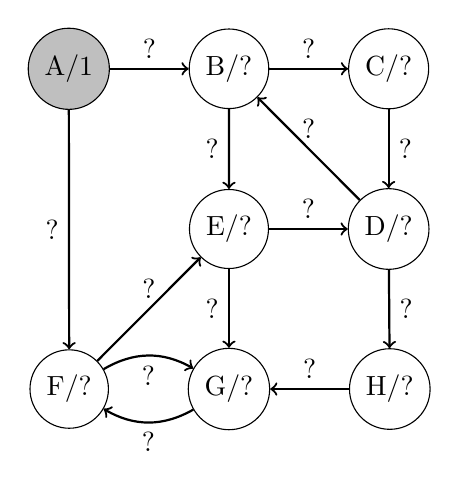
\begin{tikzpicture}[baseline=(A.north), c/.style={circle, draw}, visited/.style={fill=lightgray}]
		\node [c, visited] (A) {A/1};
		\node [c, right=of A] (B) {B/?};
		\node [c, right=of B] (C) {C/?};
		\node [c, below=of C] (D) {D/?};
		\node [c, left =of D] (E) {E/?};
		\node [c, below=of E] (G) {G/?};
		\node [c, left =of G] (F) {F/?};
		\node [c, right=of G] (H) {H/?};

		\path[->, thick] (A) edge node [above] {?} (B);
		\path[->, thick] (A) edge node [left ] {?} (F);
		\path[->, thick] (B) edge node [above] {?} (C);
		\path[->, thick] (B) edge node [left ] {?} (E);
		\path[->, thick] (C) edge node [right] {?} (D);
		\path[->, thick] (D) edge node [above] {?} (B);
		\path[->, thick] (D) edge node [right] {?} (H);
		\path[->, thick] (E) edge node [above] {?} (D);
		\path[->, thick] (E) edge node [left ] {?} (G);
		\path[->, thick] (F) edge node [above] {?} (E);
		\path[->, thick] (F) edge [bend left] node [below] {?} (G);
		\path[->, thick] (G) edge [bend left] node [below] {?} (F);
		\path[->, thick] (H) edge node [above] {?} (G);
	\end{tikzpicture}

	\item
	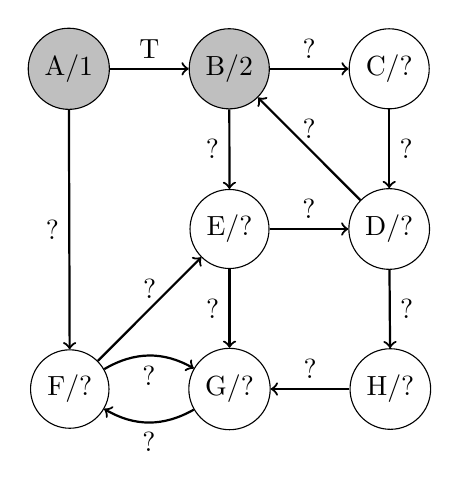
\begin{tikzpicture}[baseline=(A.north), c/.style={circle, draw}, visited/.style={fill=lightgray}]
		\node [c, visited] (A) {A/1};
		\node [c, visited, right=of A] (B) {B/2};
		\node [c, right=of B] (C) {C/?};
		\node [c, below=of C] (D) {D/?};
		\node [c, left =of D] (E) {E/?};
		\node [c, below=of E] (G) {G/?};
		\node [c, left =of G] (F) {F/?};
		\node [c, right=of G] (H) {H/?};

		\path[->, thick] (A) edge node [above] {T} (B);
		\path[->, thick] (A) edge node [left ] {?} (F);
		\path[->, thick] (B) edge node [above] {?} (C);
		\path[->, thick] (B) edge node [left ] {?} (E);
		\path[->, thick] (C) edge node [right] {?} (D);
		\path[->, thick] (D) edge node [above] {?} (B);
		\path[->, thick] (D) edge node [right] {?} (H);
		\path[->, thick] (E) edge node [above] {?} (D);
		\path[->, thick] (E) edge node [left ] {?} (G);
		\path[->, thick] (F) edge node [above] {?} (E);
		\path[->, thick] (F) edge [bend left] node [below] {?} (G);
		\path[->, thick] (G) edge [bend left] node [below] {?} (F);
		\path[->, thick] (H) edge node [above] {?} (G);
	\end{tikzpicture}

	\item
	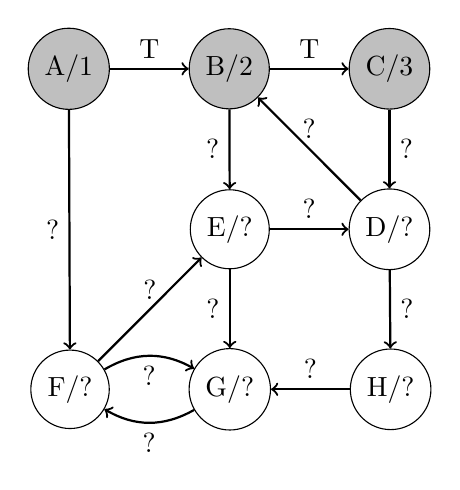
\begin{tikzpicture}[baseline=(A.north), c/.style={circle, draw}, visited/.style={fill=lightgray}]
		\node [c, visited] (A) {A/1};
		\node [c, visited, right=of A] (B) {B/2};
		\node [c, visited, right=of B] (C) {C/3};
		\node [c, below=of C] (D) {D/?};
		\node [c, left =of D] (E) {E/?};
		\node [c, below=of E] (G) {G/?};
		\node [c, left =of G] (F) {F/?};
		\node [c, right=of G] (H) {H/?};

		\path[->, thick] (A) edge node [above] {T} (B);
		\path[->, thick] (A) edge node [left ] {?} (F);
		\path[->, thick] (B) edge node [above] {T} (C);
		\path[->, thick] (B) edge node [left ] {?} (E);
		\path[->, thick] (C) edge node [right] {?} (D);
		\path[->, thick] (D) edge node [above] {?} (B);
		\path[->, thick] (D) edge node [right] {?} (H);
		\path[->, thick] (E) edge node [above] {?} (D);
		\path[->, thick] (E) edge node [left ] {?} (G);
		\path[->, thick] (F) edge node [above] {?} (E);
		\path[->, thick] (F) edge [bend left] node [below] {?} (G);
		\path[->, thick] (G) edge [bend left] node [below] {?} (F);
		\path[->, thick] (H) edge node [above] {?} (G);
	\end{tikzpicture}

	\item
	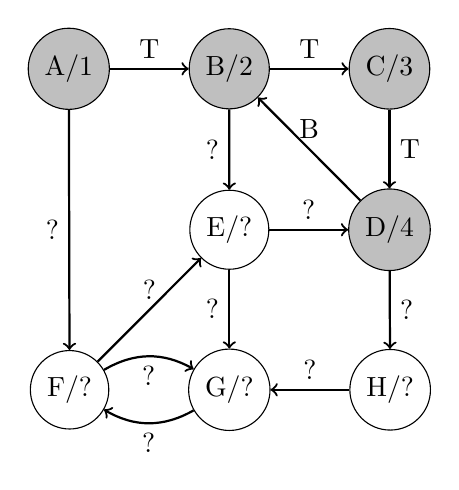
\begin{tikzpicture}[baseline=(A.north), c/.style={circle, draw}, visited/.style={fill=lightgray}]
		\node [c, visited] (A) {A/1};
		\node [c, visited, right=of A] (B) {B/2};
		\node [c, visited, right=of B] (C) {C/3};
		\node [c, visited, below=of C] (D) {D/4};
		\node [c, left =of D] (E) {E/?};
		\node [c, below=of E] (G) {G/?};
		\node [c, left =of G] (F) {F/?};
		\node [c, right=of G] (H) {H/?};

		\path[->, thick] (A) edge node [above] {T} (B);
		\path[->, thick] (A) edge node [left ] {?} (F);
		\path[->, thick] (B) edge node [above] {T} (C);
		\path[->, thick] (B) edge node [left ] {?} (E);
		\path[->, thick] (C) edge node [right] {T} (D);
		\path[->, thick] (D) edge node [above] {B} (B);
		\path[->, thick] (D) edge node [right] {?} (H);
		\path[->, thick] (E) edge node [above] {?} (D);
		\path[->, thick] (E) edge node [left ] {?} (G);
		\path[->, thick] (F) edge node [above] {?} (E);
		\path[->, thick] (F) edge [bend left] node [below] {?} (G);
		\path[->, thick] (G) edge [bend left] node [below] {?} (F);
		\path[->, thick] (H) edge node [above] {?} (G);
	\end{tikzpicture}

	\item
	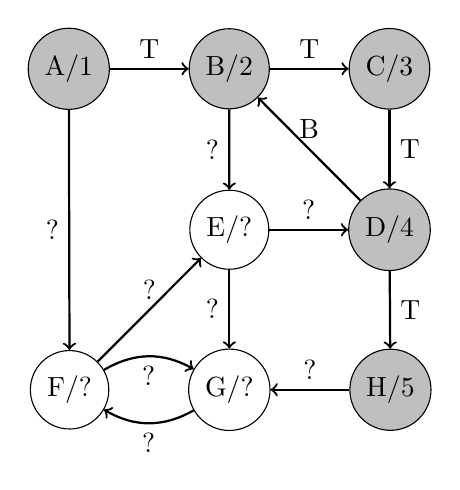
\begin{tikzpicture}[baseline=(A.north), c/.style={circle, draw}, visited/.style={fill=lightgray}]
		\node [c, visited] (A) {A/1};
		\node [c, visited, right=of A] (B) {B/2};
		\node [c, visited, right=of B] (C) {C/3};
		\node [c, visited, below=of C] (D) {D/4};
		\node [c, left =of D] (E) {E/?};
		\node [c, below=of E] (G) {G/?};
		\node [c, left =of G] (F) {F/?};
		\node [c, visited, right=of G] (H) {H/5};

		\path[->, thick] (A) edge node [above] {T} (B);
		\path[->, thick] (A) edge node [left ] {?} (F);
		\path[->, thick] (B) edge node [above] {T} (C);
		\path[->, thick] (B) edge node [left ] {?} (E);
		\path[->, thick] (C) edge node [right] {T} (D);
		\path[->, thick] (D) edge node [above] {B} (B);
		\path[->, thick] (D) edge node [right] {T} (H);
		\path[->, thick] (E) edge node [above] {?} (D);
		\path[->, thick] (E) edge node [left ] {?} (G);
		\path[->, thick] (F) edge node [above] {?} (E);
		\path[->, thick] (F) edge [bend left] node [below] {?} (G);
		\path[->, thick] (G) edge [bend left] node [below] {?} (F);
		\path[->, thick] (H) edge node [above] {?} (G);
	\end{tikzpicture}

	\item
	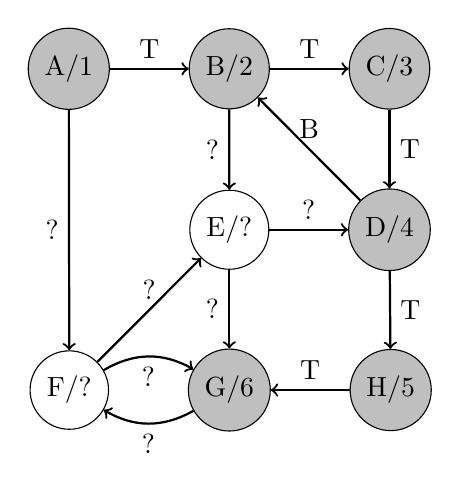
\begin{tikzpicture}[baseline=(A.north), c/.style={circle, draw}, visited/.style={fill=lightgray}]
		\node [c, visited] (A) {A/1};
		\node [c, visited, right=of A] (B) {B/2};
		\node [c, visited, right=of B] (C) {C/3};
		\node [c, visited, below=of C] (D) {D/4};
		\node [c, left =of D] (E) {E/?};
		\node [c, visited, below=of E] (G) {G/6};
		\node [c, left =of G] (F) {F/?};
		\node [c, visited, right=of G] (H) {H/5};

		\path[->, thick] (A) edge node [above] {T} (B);
		\path[->, thick] (A) edge node [left ] {?} (F);
		\path[->, thick] (B) edge node [above] {T} (C);
		\path[->, thick] (B) edge node [left ] {?} (E);
		\path[->, thick] (C) edge node [right] {T} (D);
		\path[->, thick] (D) edge node [above] {B} (B);
		\path[->, thick] (D) edge node [right] {T} (H);
		\path[->, thick] (E) edge node [above] {?} (D);
		\path[->, thick] (E) edge node [left ] {?} (G);
		\path[->, thick] (F) edge node [above] {?} (E);
		\path[->, thick] (F) edge [bend left] node [below] {?} (G);
		\path[->, thick] (G) edge [bend left] node [below] {?} (F);
		\path[->, thick] (H) edge node [above] {T} (G);
	\end{tikzpicture}

	\item
	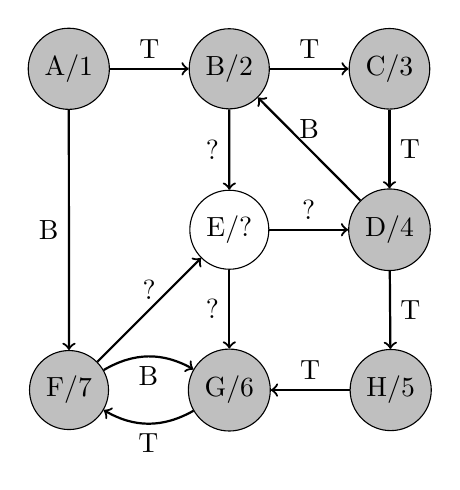
\begin{tikzpicture}[baseline=(A.north), c/.style={circle, draw}, visited/.style={fill=lightgray}]
		\node [c, visited] (A) {A/1};
		\node [c, visited, right=of A] (B) {B/2};
		\node [c, visited, right=of B] (C) {C/3};
		\node [c, visited, below=of C] (D) {D/4};
		\node [c, left =of D] (E) {E/?};
		\node [c, visited, below=of E] (G) {G/6};
		\node [c, visited, left =of G] (F) {F/7};
		\node [c, visited, right=of G] (H) {H/5};

		\path[->, thick] (A) edge node [above] {T} (B);
		\path[->, thick] (A) edge node [left ] {B} (F);
		\path[->, thick] (B) edge node [above] {T} (C);
		\path[->, thick] (B) edge node [left ] {?} (E);
		\path[->, thick] (C) edge node [right] {T} (D);
		\path[->, thick] (D) edge node [above] {B} (B);
		\path[->, thick] (D) edge node [right] {T} (H);
		\path[->, thick] (E) edge node [above] {?} (D);
		\path[->, thick] (E) edge node [left ] {?} (G);
		\path[->, thick] (F) edge node [above] {?} (E);
		\path[->, thick] (F) edge [bend left] node [below] {B} (G);
		\path[->, thick] (G) edge [bend left] node [below] {T} (F);
		\path[->, thick] (H) edge node [above] {T} (G);
	\end{tikzpicture}

	\item
	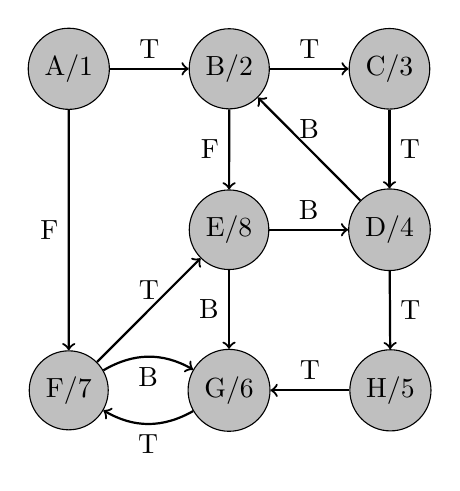
\begin{tikzpicture}[baseline=(A.north), c/.style={circle, draw}, visited/.style={fill=lightgray}]
		\node [c, visited] (A) {A/1};
		\node [c, visited, right=of A] (B) {B/2};
		\node [c, visited, right=of B] (C) {C/3};
		\node [c, visited, below=of C] (D) {D/4};
		\node [c, visited, left =of D] (E) {E/8};
		\node [c, visited, below=of E] (G) {G/6};
		\node [c, visited, left =of G] (F) {F/7};
		\node [c, visited, right=of G] (H) {H/5};

		\path[->, thick] (A) edge node [above] {T} (B);
		\path[->, thick] (A) edge node [left ] {F} (F);
		\path[->, thick] (B) edge node [above] {T} (C);
		\path[->, thick] (B) edge node [left ] {F} (E);
		\path[->, thick] (C) edge node [right] {T} (D);
		\path[->, thick] (D) edge node [above] {B} (B);
		\path[->, thick] (D) edge node [right] {T} (H);
		\path[->, thick] (E) edge node [above] {B} (D);
		\path[->, thick] (E) edge node [left ] {B} (G);
		\path[->, thick] (F) edge node [above] {T} (E);
		\path[->, thick] (F) edge [bend left] node [below] {B} (G);
		\path[->, thick] (G) edge [bend left] node [below] {T} (F);
		\path[->, thick] (H) edge node [above] {T} (G);
	\end{tikzpicture}
\end{enumerate}

\section{} %2
You can find the minimum number of semesters necessary by using a kind of reverse BFS.

\begin{enumerate}
	\item Initialize the semester counter to 1.
	\item Mark nodes with out-degree 0 (the final courses) as visited.
	\item \label{loop} Follow the ingoing edges of the last visited nodes and mark their origin nodes as visited when all of their outgoing edges connect to visited nodes.
	\item Increment the semester counter.
	\item If any of these nodes have an in-degree $> 0$, go to \ref{loop}, else go to \ref{end}
	\item \label{end} Return the semester counter.
\end{enumerate}

Example:

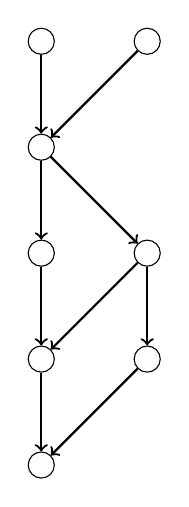
\begin{tikzpicture}[c/.style={circle, draw}, v/.style={fill=gray}]
	\node[c] (a) {};
	\node[c, right=of a] (b) {};
	\node[c, below=of a] (c) {};
	\node[c, below=of c] (d) {};
	\node[c, right=of d] (e) {};
	\node[c, below=of d] (f) {};
	\node[c, below=of e] (g) {};
	\node[c, below=of f] (h) {};

	\path[->, thick] (a) edge (c);
	\path[->, thick] (b) edge (c);
	\path[->, thick] (c) edge (d);
	\path[->, thick] (c) edge (e);
	\path[->, thick] (d) edge (f);
	\path[->, thick] (e) edge (f);
	\path[->, thick] (e) edge (g);
	\path[->, thick] (f) edge (h);
	\path[->, thick] (g) edge (h);
\end{tikzpicture}

\begin{enumerate}
	\item
	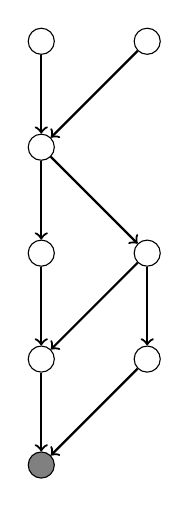
\begin{tikzpicture}[baseline=(a.south), c/.style={circle, draw}, v/.style={fill=gray}]
		\node[c] (a) {};
		\node[c, right=of a] (b) {};
		\node[c, below=of a] (c) {};
		\node[c, below=of c] (d) {};
		\node[c, right=of d] (e) {};
		\node[c, below=of d] (f) {};
		\node[c, below=of e] (g) {};
		\node[c, v, below=of f] (h) {};

		\path[->, thick] (a) edge (c);
		\path[->, thick] (b) edge (c);
		\path[->, thick] (c) edge (d);
		\path[->, thick] (c) edge (e);
		\path[->, thick] (d) edge (f);
		\path[->, thick] (e) edge (f);
		\path[->, thick] (e) edge (g);
		\path[->, thick] (f) edge (h);
		\path[->, thick] (g) edge (h);
	\end{tikzpicture}
	Semester counter = 1

	\item
	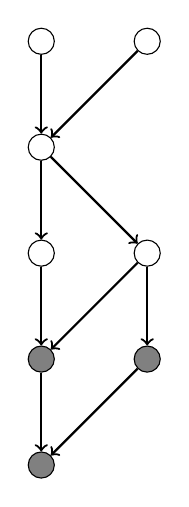
\begin{tikzpicture}[baseline=(a.south), c/.style={circle, draw}, v/.style={fill=gray}]
		\node[c] (a) {};
		\node[c, right=of a] (b) {};
		\node[c, below=of a] (c) {};
		\node[c, below=of c] (d) {};
		\node[c, right=of d] (e) {};
		\node[c, v, below=of d] (f) {};
		\node[c, v, below=of e] (g) {};
		\node[c, v, below=of f] (h) {};

		\path[->, thick] (a) edge (c);
		\path[->, thick] (b) edge (c);
		\path[->, thick] (c) edge (d);
		\path[->, thick] (c) edge (e);
		\path[->, thick] (d) edge (f);
		\path[->, thick] (e) edge (f);
		\path[->, thick] (e) edge (g);
		\path[->, thick] (f) edge (h);
		\path[->, thick] (g) edge (h);
	\end{tikzpicture}
	Semester counter = 2

	\item
	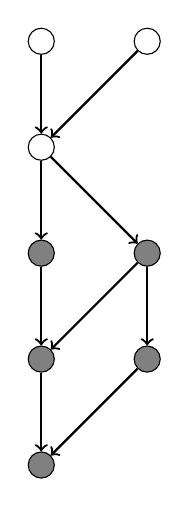
\begin{tikzpicture}[baseline=(a.south), c/.style={circle, draw}, v/.style={fill=gray}]
		\node[c] (a) {};
		\node[c, right=of a] (b) {};
		\node[c, below=of a] (c) {};
		\node[c, v, below=of c] (d) {};
		\node[c, v, right=of d] (e) {};
		\node[c, v, below=of d] (f) {};
		\node[c, v, below=of e] (g) {};
		\node[c, v, below=of f] (h) {};

		\path[->, thick] (a) edge (c);
		\path[->, thick] (b) edge (c);
		\path[->, thick] (c) edge (d);
		\path[->, thick] (c) edge (e);
		\path[->, thick] (d) edge (f);
		\path[->, thick] (e) edge (f);
		\path[->, thick] (e) edge (g);
		\path[->, thick] (f) edge (h);
		\path[->, thick] (g) edge (h);
	\end{tikzpicture}
	Semester counter = 3

	\item
	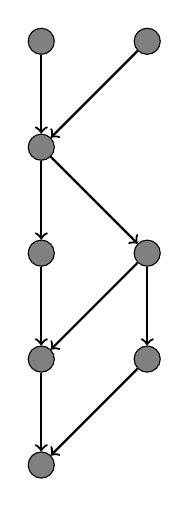
\begin{tikzpicture}[baseline=(a.south), c/.style={circle, draw}, v/.style={fill=gray}]
		\node[c, v] (a) {};
		\node[c, v, right=of a] (b) {};
		\node[c, v, below=of a] (c) {};
		\node[c, v, below=of c] (d) {};
		\node[c, v, right=of d] (e) {};
		\node[c, v, below=of d] (f) {};
		\node[c, v, below=of e] (g) {};
		\node[c, v, below=of f] (h) {};

		\path[->, thick] (a) edge (c);
		\path[->, thick] (b) edge (c);
		\path[->, thick] (c) edge (d);
		\path[->, thick] (c) edge (e);
		\path[->, thick] (d) edge (f);
		\path[->, thick] (e) edge (f);
		\path[->, thick] (e) edge (g);
		\path[->, thick] (f) edge (h);
		\path[->, thick] (g) edge (h);
	\end{tikzpicture}
	Semester counter = 5
\end{enumerate}

You need at least 5 semesters to take all courses in this example.

\section{} %3
\section{} %4
Given here is an implementation of an algorithm to check for a universal sink in $O(n)$ time written in Python:

\lstinputlisting[language=Python]{code/universal_sink.py}

Usage example:

\begin{lstlisting}[language=Python]
v = matrix("""
0 1 0 0;
0 0 0 0;
0 1 0 0;
1 1 1 0
""")
print(contains_universal_sink(v)) # True

v[1, 1] = 1
print(contains_universal_sink(v)) # False
\end{lstlisting}

This algorithm uses the adjacency matrix of a given graph to check if there exists a universal sink in the graph.
It first checks the values in the column for the first node.
If the column consists of only zeros, this node is the only one possible which could be a universal sink.
So the algorithm returns the node index and checks with the function $is_sink()$ if this node is indeed an universal sink.
If this node is not an universal sink, there is none in the graph.

If the first column contains a 1, it means that the out-degree of that node is not 0, so this node cannot be a universal sink.
So the if-statement is true thus the row is incremented.
Because the first node was not the universal sink, we assume that the second node has an input from the first node.
If we encounter another 1 in the column of node 2, this node cannot be the universal sink either so we move to the next column thus to the next possible node.

This algorithm assumes that there exists a universal sink in the graph and then searches for the node which has the highest chance of being an universal sink.
If the returned node is not a universal sink, then no other node is, thus the algorithm returns false.

Because at each iteration of the while-loop, we either increment the row or the column, until one of them reaches n. The while-loop is executed at most $2n$ times.
After the loop the $is_sink()$-function is executed once which takes another $n$ steps.
Thus this algorithm takes in total $3n$ time, so it has a time complexity of $O(n)$.

\section{} %5
Given a graph $G = (V, E)$ we want to check whether there is a vertex $s \in V$ from which all other vertices are reachable.

First we find the strongly connected components using, for example, Kosaraju's algorithm, or Tarjan's algorithm.

If there is exactly one strongly connected component with no incoming edges, then all of its vertices can reach any other vertex. So there exists an $s$.

If there is more than one strongly connected component with no incoming edges, then there can be no $s$.

\section{} %6
To run in $O(|V| + |E|)$ each vertex and each edge must be visited a constant amount of times.

This can be done with Kahn's algorithm which visits every edge and vertex once, then deletes it from the graph. This is the algorithm taken from Wikipedia:

\begin{lstlisting}
L <- Empty list that will contain the sorted elements
S <- Set of all nodes with no incoming edges
while S is non-empty do
    remove a node n from S
    add n to tail of L
    for each node m with an edge e from n to m do
        remove edge e from the graph
        if m has no other incoming edges then
            insert m into S
if graph has edges then
    return error (graph has at least one cycle)
else
    return L (a topologically sorted order)
\end{lstlisting}
(https://en.wikipedia.org/wiki/Topological\_sorting\#Kahn.27s\_algorithm)

$S$ can be constructed in $O(|V| + |E|)$ by making a copy $S$ of $V$ (takes $O(|V|)$) and iterating over $E$, removing every $s \in S$ for which $(v, s) \in E, v\in V$ (takes $O(|E|)$). (This assumes $O(1)$ for insertion and deletion on the set which can be achieved by using a hash set.)

If we do this and then use it to run Kahn's algorithm we end up visiting each vertex, and each edge twice. $O(2(|V| + |E|)) = O(|V| + |E|)$.

\end{document}
